% Copyright 2014 by Damien Thiriet
%
% This work may be distributed and/or modified under the
% conditions of the LaTeX Project Public License, either version 1.3
% of this license or (at your option) any later version.
% The latest version of this license is in
% http://www.latex-project.org/lppl.txt
% and version 1.3 or later is part of all distributions of LaTeX
% version 2005/12/01 or later.
%
% This work has the LPPL maintenance status `maintained'.
% 
% The Current Maintainer of this work is Damien Thiriet
%
% This work consists of the files beamerdarkthemesuserguide.tex,
% beamerdarkthemesuserguide.pdf, beamercolorthemecormorant.sty,
% beamercolorthemefrigatebird.sty, beamercolorthememagpie.sty,
% dahut.jpg, img_5630.jpg, example.tex, frigatebirdexampletree.pdf,
% frigatebirdexampledefault.pdf, frigatebirdexamplesidebar.pdf,
% frigatebirdexampleinfolines.pdf, cormorantexampledefault.pdf,
% cormorantexamplesidebar.pdf, cormorantexampleinfolines.pdf,
% cormorantexampletree.pdf, magpieexampledefault.pdf,
% magpieexamplesidebar.pdf, magpieexampleinfolines.pdf,
% magpieexampletree.pdf, makeexamples.sh
% 
% This file is licended CC-BY version 4.0 or later.
% You will find a copy of this licence in
% http://creativecommons.org/licenses/by/4.0/legalcode
%
% img_5630.jpg was taken by Damien Thiriet in the nice Dolina Pięciu
% Stawów near Zakopane, Poland. img_5630.jpg and dahut.jpg and
% example.tex are licenced CC-BY version 4.0 or later.
%
% makeexamples.sh is based upon beamerthemesmakeexample.sh, a file that
% could be found in beamer official doc in 2013 (scripts are nowadays
% part of beamer Makefile)
% 
% beamercolorthemeseahorse.sty was used as a canvas 
% when coding beamercolorthememagpie.sty first version.
%
% Package version 0.4.1, 2014-09-03

\documentclass{beamer}

\usecolortheme{\colorname}
\useoutertheme{\outername}

\usepackage{polyglossia}

\title{Le dahut}
\subtitle{Précis de zoologie avec traité de chasse}

\author[Radin]{Ethiem Radin}
\institute[Univ. Gévaudan]{UFR de Biologie\\ Université du Gévaudan}
\date[MDCCXLVI]{Rencontres Quinte Essence, MDCCXLVI}
\logo{
\includegraphics[width=1.3cm]{ccby.png}}

\begin{document}

\begin{frame}
  \titlepage
  \tableofcontents
\end{frame}

\section{Du dahut}
\subsection{Spécificité}

\begin{frame}
  \frametitle{Une espèce montagnarde rare}

  \begin{block}{Dahut (\emph{rupicapra armoricanis})}
     Nette dissymétrie longitudinale des membres latéraux.
  \end{block}
  \begin{exampleblock}{Précisions}
    \begin{description}
       \item[taille] variable selon les observateurs;
       \item[alimentation] longs jeûnes : on ne l’a jamais vu se nourrir…
       \item[instinct grégaire] nul ; réputé solitaire.
    \end{description}
  \end{exampleblock}
\end{frame}

\subsection{Environnement}


\begin{frame}
   \frametitle{Un document exceptionnel}
   \framesubtitle{Gromsoław Krótkowidz, \emph{Paysage au dahut}, huile sur toile, 1887}
   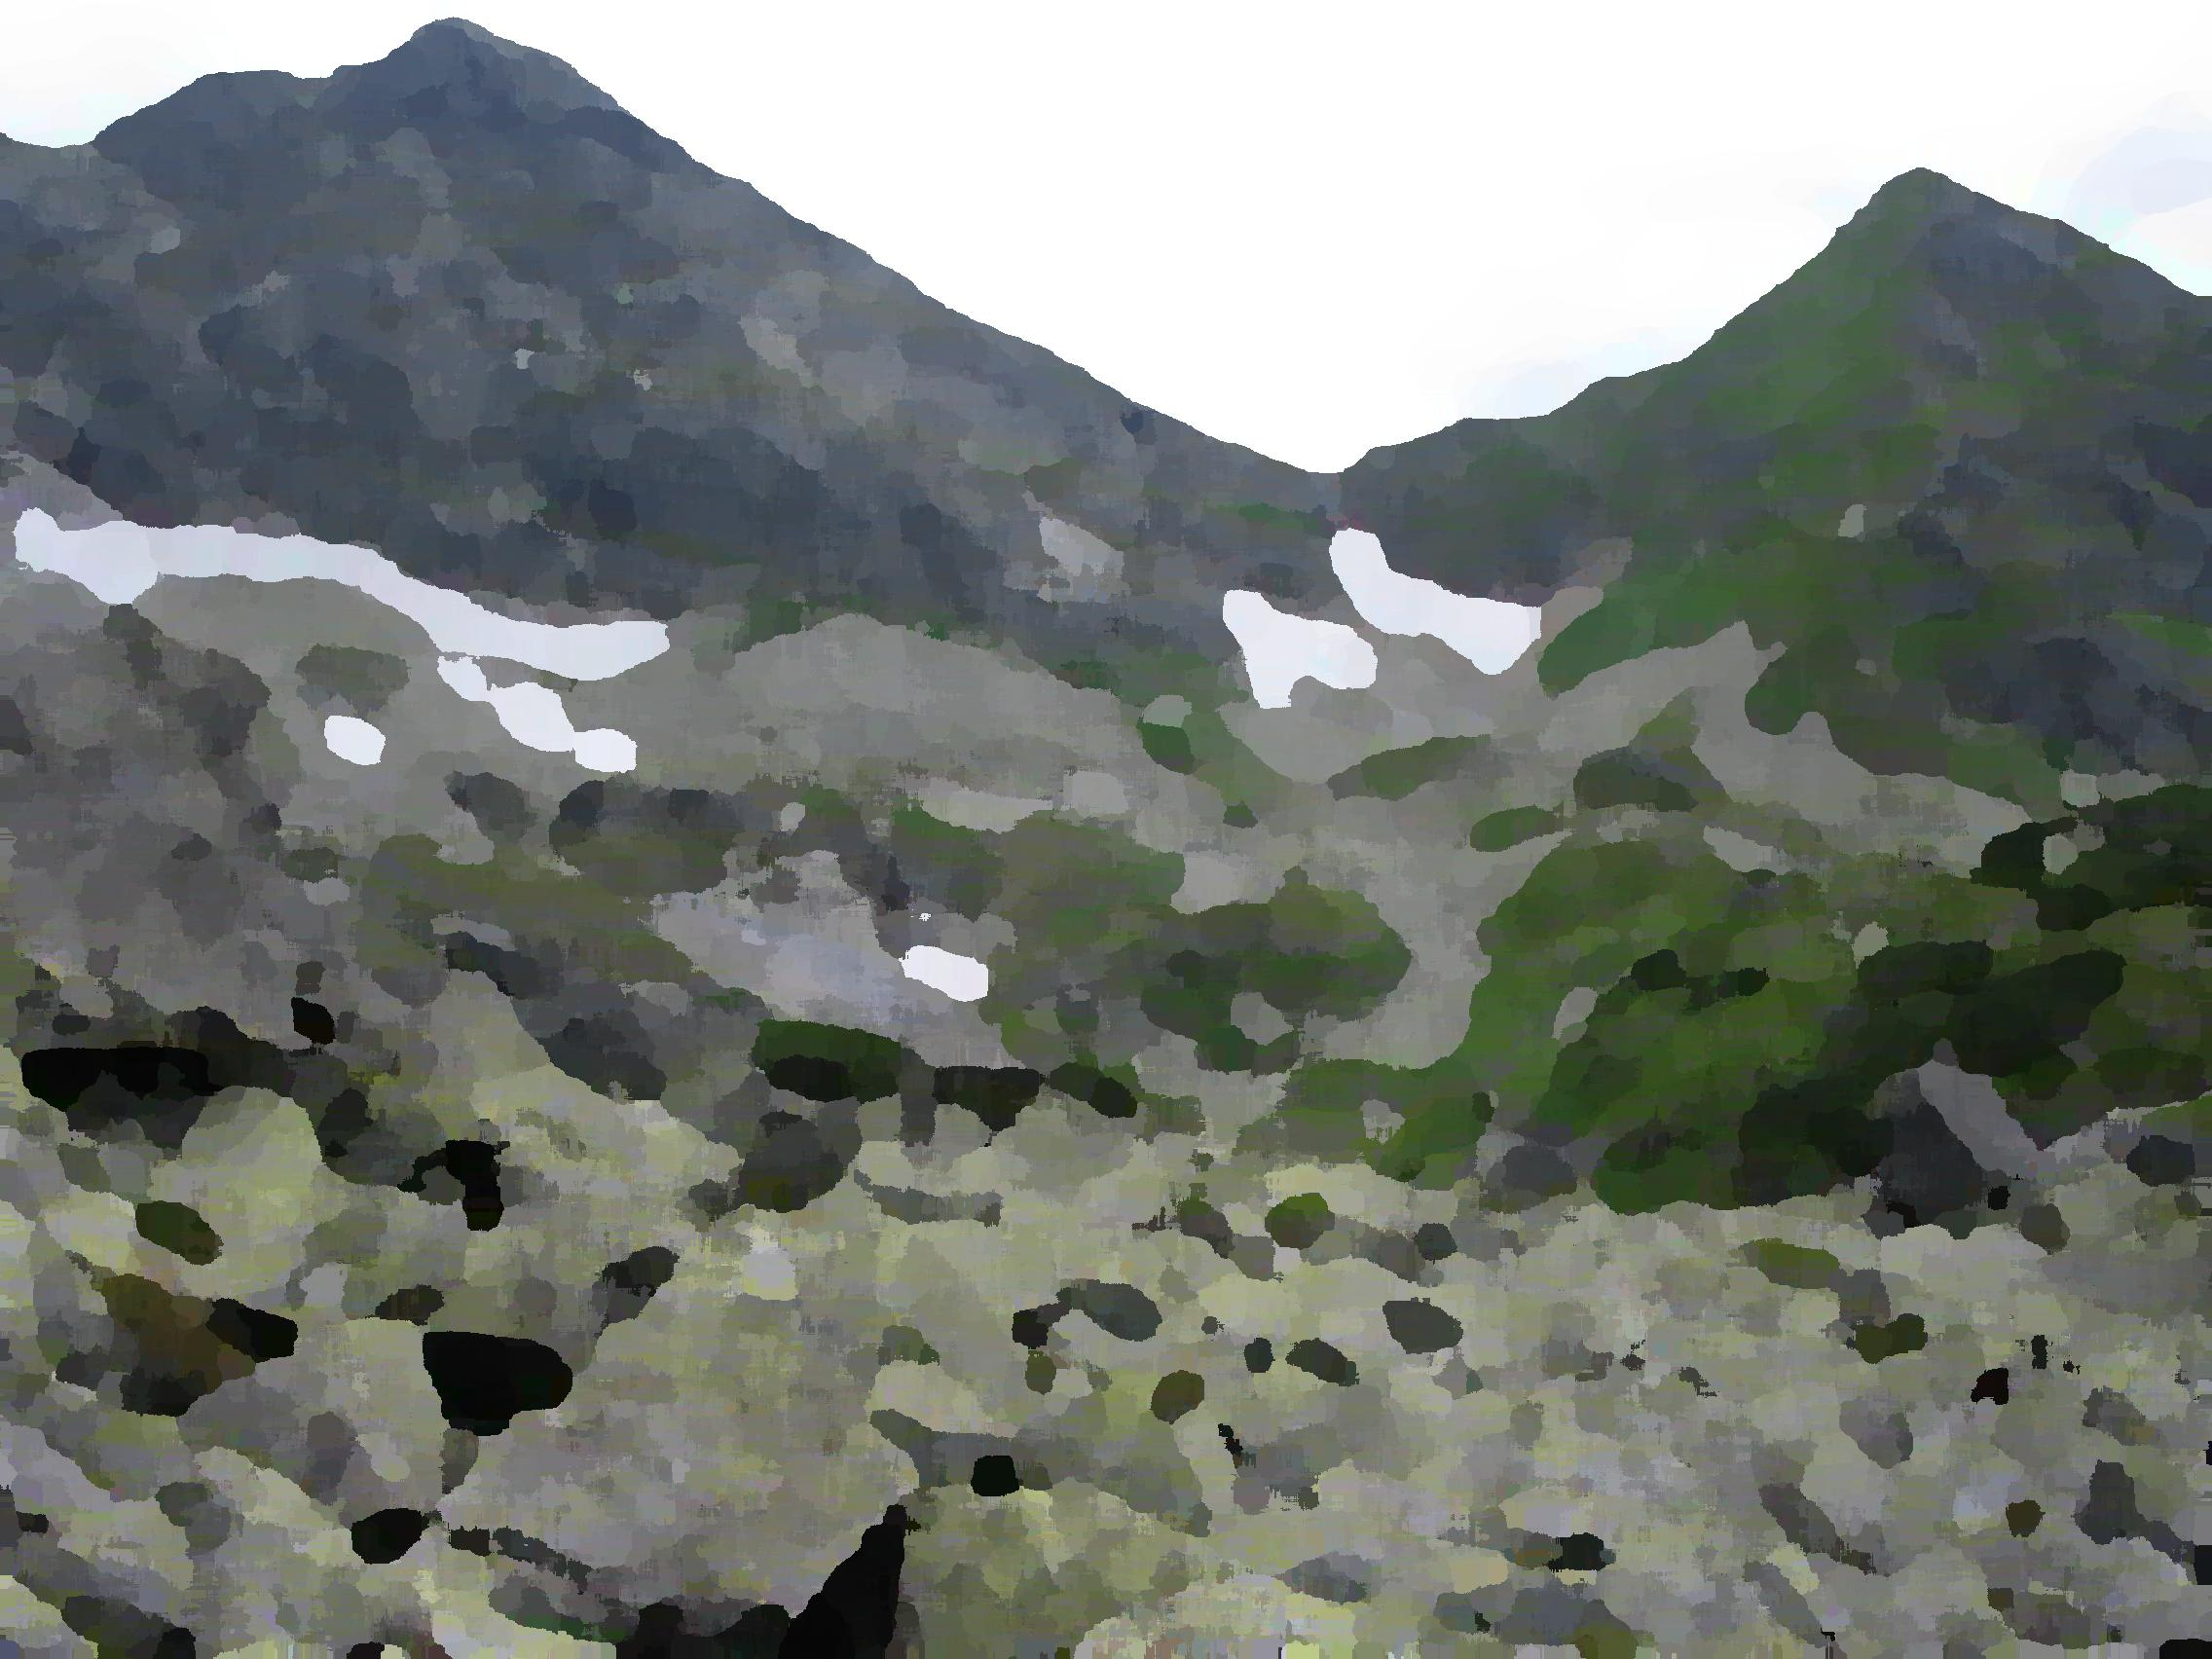
\includegraphics[width=.7\linewidth]{dahut.jpg}

   Cracovie, musée Jan Stanisławski.
\end{frame}

\section{Traité de chasse}

\begin{frame}
   \frametitle{Le traité de chasse}
   
   \begin{itemize}
      \item \structure{Attraper} un dahut demande \alert{beaucoup d’expérience}… 
      \item Il faut retourner l’animal.
   \end{itemize}
\end{frame}


\end{document}
